% File name: datalogger/Reports/Final_Report_Andy.tex
% Final report for datalogger project
% Author: adh
% Date: Mon 03 Jun 2013 11:51

\documentclass[a4paper,10pt]{article}  % Standard document class
\usepackage[english]{babel}            % Set document language
\usepackage{fullpage}                  % Set up page for small margins etc

\usepackage{todonotes}

\usepackage{graphicx}                  % For including images in document
\usepackage{placeins}                  % Allows use of \FloatBarrier
% to avoid images or tables
% moving into next section
\usepackage{subfig}                    % For subfigures...

\usepackage{amsmath}                   % For improving maths/formula typesetting
\usepackage{tabularx}                  % Table changing package

\usepackage{algpseudocode}             % For producing algorithms/flowcharts

\usepackage{color}
\definecolor{grey}{rgb}{0.5,0.5,0.5}

\usepackage{listings}                  % For including source code in document
\lstset{
  basicstyle = \footnotesize\ttfamily,
  commentstyle = \color{grey},
  keepspaces = true,
  keywordstyle = \color{blue},
  language = C++,
  numbers = left,
  numbersep=5pt,
  numberstyle=\tiny\color{grey},
  stepnumber=5,
  tabsize=2,
}

\usepackage{url}

% Provide command for scientific notation
\providecommand{\e}[1]{\ensuremath{\times10^{#1}}}
\providecommand{\degrees}{\ensuremath{^{\circ}}}

% Define title here:
\title{Project SB3: Data Logger\\
       Package Environment Monitoring\\
       Final Report}
\author{Andrew Holt\\
        ah635\\
        Team 6\\
        Emmanuel}
\date{06 June 2013}

\begin{document}

% generate title
\maketitle

\vspace{\stretch{1}}

\begin{center}
  \includegraphics[width=0.5\textwidth]{damaged_parcel.jpg}
\end{center}

\vspace{\stretch{2}}

\begin{abstract}
An opportunity was noticed to develop a product for tracking
the environmental conditions of a package in transit. A prototype
system has been produced, requiring hardware, firmware and software
development. The prototype has been found to show good potential, but
requires some refining before it could become a commercially viable
product. The project has been enjoyable and it has been rewarding to
apply some of the knowledge gained in lecture courses to real product
development.
\end{abstract}

\newpage

\tableofcontents
\vspace{\stretch{1}}
\listoffigures
\listoftables

\newpage

\section{Introduction}
\label{sec:introduction}

The express delivery industry is one of the fastest growing industries
in the world today. In 2003, the industry made a direct contribution
of US\$64 billion to worldwide GDP, and has been growing by around 8\%
per year since \cite{OEF2005}. However, customers have very little
information of the environmental and handling conditions their package
has been subject to during its transit. When shipping fragile or
sensitive products, the conditions that the parcel is subject to may
be critical in the integrity of the product. The two major issues here
are:
\begin{enumerate}
\item Fragile goods which arrive broken: it is desirable to determine
  whether the package has been mishandled, and if so by whom.
\item Perishable goods: if they have been subjected to conditions
  outside of sensitive temperature and humidity limits they will have
  a shorted shelf life. This may not be obvious upon inspection of the
  goods, so detailed condition tracking is required.
\end{enumerate}
While products have been around for a while to carry out this type of
tracking on shipping containers, the same problem applies to smaller
and domestic packages too. In the past six months, two large companies
have announced products to achieve this, but it is clearly an emerging
market and a good product launched now could have a great chance of
success. One of these recent products, ``SenseAware''\cite{SA_PR} by
FedEx Corporation, is already released and available however this is
only available on a select number of carriers and services and is a
business level product, not suited for everyday or relatively low
value package monitoring. An alternative is the ``DropTag'' system
recently announced by Cambridge Consultants \cite{DT_PR}, however this
system is not yet at the commercial release stage.

With a problem identified and a solution required, as well as a clear
business opportunity due to the interest in development from other
companies, product development was begun.

\section{Overview}
\label{sec:overview}

In order to effectively track the condition of a parcel during
transit, the final product was clearly required to be cheap, low power
and physically small and robust. For this project, a simple prototype
was to be developed, which if successful could be miniaturised and
fabricated for the final product.

\subsection{Summary of Design}
\label{sec:summary-design}

The first stage of the design process was to evaluate which quantities
should be measured and logged. The key environmental variables would
be temperature and humidity. Vibration, orientation and shocks would
also be required to understand the handling and transport
conditions. GPS tracking would also be useful, but it was decided to
focus on the other five initially as GPS could be relatively easily
included with a dedicated GPS chip communicating over the I$^2$C
protocol, and GPS reception may be limited at many points during
transit.

The product would clearly be required to work without being plugged in
to a computer, so a standalone mode would be developed. It would be
useful for development, debugging and testing to operate with instant
feedback from the computer system, so a linked mode was also
developed.

To ensure long term operation, on-board memory would be required, so an
EEPROM was used for data storage in the standalone mode. This would
also require a battery supply.

Some kind of on-board display would also be useful on the board, for
monitoring, debugging and status display, so an LCD screen was used
along with five LEDs.

The platform choices were specified in the project requirements, so
the project was to be developed for the STM32F100 ARM Cortex
microcontroller and a PC running the Windows operating system. The key
design areas would therefore be hardware, firmware and software. The
budget was generous for the development board so cost was not really
an issue, however to achieve a commercial product, the cost and size
would need to be reduced. This could be achieved by miniaturising, as
surface mount components tend to be cheaper; use of a cheaper
microcontroller (which wouldn't need the development features of the
STM); and economies of scale in a full production product.

The block diagram for the system is shown in figure
\ref{fig:sysblkdgrm}.
\begin{figure}[htb]
  \begin{center}
    \includegraphics[width=1.0\textwidth]{System_diagram.png}
  \end{center}
  \caption{Overall system block diagram}
  \label{fig:sysblkdgrm}
\end{figure}

\subsection{Project Management}
\label{sec:project-management}

The project was divided between the two team members. It was decided
that James would write the firmware for the microcontroller, Andrew
would write the software for the computer and the hardware design was
to be shared. The general development plan was to start by making a
basic but working system and gradually adding features and complexity
upon the existing system. This ensured that we would have a fully
operational product, if not with every desired feature, by the end of
the project, and would also allow the simpler parts to be used in
testing more complex parts.

Initially basic hardware circuits were designed and built. The firmware
and software were then developed. The hardware circuits were highly
useful in testing the firmware, but in writing the firmware, flaws in
the circuit designs became apparent, such as the initial plan to use a
simple charge-discharge of the humidity sensor. For this reason, the
humidity sensor circuit was updated during the project.

\section{Design}
\label{sec:design}

A brief overview of the design has been given in section
\ref{sec:summary-design}. This section gives technical detail about
the parts of the system which I designed. The other parts are detailed
in James' report.

A photo of the completed hardware is shown in figure \ref{fig:boardphoto}.
\begin{figure}[!htb]
  \begin{center}
    \includegraphics[width=0.8\textwidth]{completedboard_annotated.png}
  \end{center}
  \caption{Completed data logger board.}
  \label{fig:boardphoto}
\end{figure}

\subsection{Hardware}
\label{sec:hardware}

In order to measure temperature, it was decided to use a
thermistor. Thermistors have some advantages over other temperature
measurement devices such as thermocouples, resonant crystal
thermometers and diode junction voltage measurement such as \cite{HH}:
\begin{enumerate}
  \item The dependant quantity is very easy to measure.
  \item Large change in measured quantity (thousands of ohms, compared
    to millivolt changes in thermocouples and diode junctions), meaning
    low demands are placed on the analogue circuitry.
  \item Inexpensive.
  \item Good stability.
  \item Circuit can easily be designed to give very linear output,
    making the digital conversion to temperature straightforward.
\end{enumerate}
With these considerations, an ND06P00103K NTC $10\,\mathrm{k\Omega}$
thermistor from AVX was selected, based on price and good electrical
characteristics for the application requirements. 

An analogue signal processing circuit was required to process the
output from the thermistor to a signal usable by the microcontroller
analogue-to-digital converter (ADC). This required a signal in the
range of $0-3.3\,\mathrm{V}$.

The thermistor was placed in a voltage divider circuit with a series
$10\,\mathrm{k\Omega}$ resistor. This was selected to linearize the
temperature curve. This combination gives a response linear to within
$1\,\mathrm{\%}$ from $0\ \mathrm{to}\ 40\,\mathrm{\degrees C}$ and
$3\,\mathrm{\%}$ between $-10\ \mathrm{and}\ 50\,\mathrm{\degrees
  C}$\cite{HH}. This voltage divider operates from a 3.3V rail, ensuring that
the input to the next stage will always lie within its supply
rails. At this supply level, the maximum power dissipation through the
thermistor was calculated as $3.3\,\mathrm{mW}$ at
$50\,\mathrm{\degrees C}$. This is well below the maximum dissipation
for the thermistor of $0.71\,\mathrm{mW}$, so will not have a
noticeable affect on the temperature measurement.

The output from the voltage divider drives an op-amp non-inverting
amplifier circuit. The voltage divider has relatively high output
resistance, so use of a non-inverting op-amp configuration ensures a
very large input resistance ($\sim 10^{13}\, \mathrm{\Omega}$),
avoiding loading on the measurement circuit.

The non-inverting amplifier is slightly non-standard due to a non-zero
reference voltage on the inverting terminal. This is selected to give
the same output as the thermistor setup at the low end of its
response, which was selected as $-20\,\mathrm{\degrees C}$ as this
will lie well below the temperature a package would expect to
experience in transit and is at the limit of the linear response. This
reference voltage was found to be $0.79\,\mathrm{V}$, so is generated
using a series combination of $22\,\mathrm{k \Omega}$ and two
$10\,\mathrm{k \Omega}$ resistors, giving a very close voltage match
with standard resistor values.

The gain was then calculated to produce a $3.3\,\mathrm{V}$ output
swing over the input range to be received, and the gain required was
found to be 1.47. This was achieved in the non-inverting amplifier
using standard resistor values of $56\ \mathrm{and}\ 120\,\mathrm{k
  \Omega}$.

The output swing was chosen to span the full supply level of
$0-3.3\,\mathrm{V}$ as the op-amp used provides very good rail-to-rail
operation, and the extremes of the working temperature range are both
unlikely to experienced and reaching the limits of the linear response
from the thermistor. For the package tracking application, it is not
critical to know how far beyond these limits the temperature has
reached, so a simple saturating output is sufficient. This allows the
ADC to operate with maximum precision.

The circuit diagram for the temperature monitoring circuit is shown in
appendix \ref{sec:source-code-circuit}, figure \ref{fig:tempcct}.

A filter could easily have been implemented in the op-amp to avoid
noise, since the signal is of very low frequency. However, the output
was found to be very stable without filtering, so filtering was
avoided for the sake of simplicity.

\subsection{Software}
\label{sec:software}

It was suggested to use the National Instruments ``LabWindows/CVI''
package for developing the PC software and graphical user interface
(gui), however it was decided to eschew this in favour of developing
in C++ and the wxWidgets cross platform gui toolkit. The reasons for
this were:
\begin{enumerate}
\item LabWindows is a highly specialist and proprietary development
  package. While it is simple to use and fast to setup, we found it
  unlikely that we would use it again in the future.
\item LabWindows is fairly limited in scope of what can be achieved,
  whereas wxWidgets and C++ allow pretty much anything to be achieved.
\item Our other project was using C++ and wxWidgets, so it was a
  simpler option to only learn one package, rather than one per project.
\item Past experience of coding in C++ could be utilised, whereas
  LabWindows relies on C which I have very little experience of.
\end{enumerate}

There are three main components to the software development. The
back end functionality required serial port communications and
communications protocols with the microcontroller. The front end required a simple
user interface to display the logged data and control the
microcontroller functions. See appendix \ref{sec:source-code-circuit}
for a full code listing.

The actual data transmission is handled by the serial port
library.

The sending of packets to and from the serial port for the
microcontroller are handled by the communications level, which
provides an interface between the application and the actual data, so
the user and user interface level do not depend on the communications
system. This is advantageous as it means the top level application is
independent of the communication medium, and could be converted to use
USB or wifi without modifying the user application. It also simplifies
the functions required in the user application as they do not directly
handle the raw data, but instead use more user/programmer friendly
data structures.

On top of the communications layer is the application and user
interface layer. These allow easy and logical viewing and
understanding of commands to be sent and data received by the
computer.

This hierarchical structure is shown in figure
\ref{fig:commsprotocol}. The layers map very roughly onto the Open
Systems Interconnect (OSI) reference model. The user interface
performs the duties of layer 7 (application). The communications layer
is similar to layer 6 (presentation), while the rs232 library spans
levels 4 and 5 (transport and session layers, respectively). The lower
layers are defined by the RS232 protocol.

\begin{figure}[!htb]
  \begin{center}
    \includegraphics[width=0.7\textwidth]{CommunicationsProtocol.png}
  \end{center}
  \caption{Communications stack showing interaction of each layer.}
  \label{fig:commsprotocol}
\end{figure}

\subsubsection{Serial Port Communications}

The files \texttt{rs232.cpp} and \texttt{rs232.h} contain functions for
sending and receiving data from the serial port. These were found
online \cite{rs232_lib}, released under the GNU General Public
Licence. (See section \ref{sec:probl-enco-techn} for more details.)

The important functions provided by this software is are:
\begin{description}
  \item[\texttt{RS\_232\_OpenComport()}]
    This sets up the connection with the serial port to be used,
    setting up a two way communications link to the microcontroller.
  \item[\texttt{RS\_232\_CloseComport()}] Closes the connection to the
    serial port at the end of the operation.
  \item[\texttt{RS\_232\_PollComport()}] Reads data that has been sent
    by the microcontroller to the computer.
  \item[\texttt{RS\_232\_SendBuf()}] Writes to the serial port to send
    commands to the microcontroller.
\end{description}

These functions were all provided directly by the software found
online, which greatly simplified the serial port reading.

\subsubsection{Communications}

The functions provided in the RS\_232 library are very low level, and
perform sending and receiving of individual bytes. For the user
interface, it is useful to have a high level data structure, rather
than dealing with individual bytes of data. The files
\texttt{comms.cpp} and \texttt{comms.h} provide the means to do
this. The functions here call the functions in \texttt{rs232.cpp}. It
converts the user commands into the required bytes to send to the
microcontroller, and organises the returned data into a
\texttt{vector} data structure.

This level provides functions to be called by the data logger
application:
\begin{description}
  \item[\texttt{RS232\_Init()}] Opens the required comport to
    establish a link with the microcontroller.
  \item[\texttt{RS232\_Close()}] Closes the opened comport.
  \item[\texttt{send\_command()}] Sends a command to the
    microcontroller by writing to the serial port buffer (uses the
    \texttt{SendBuf} function).
  \item[\texttt{read\_eeprom\_data()}] Reads data stored in the EEPROM
    into a \texttt{vector}.
  \item[\texttt{get\_Readings()}] Receives the data sent by the
    microcontroller in linked mode and stores it in a vector.
\end{description}

\subsubsection{User Interface}

The top level of the PC system is the user interface, which allows the
user to interact with the system in an intuitive and non-technical
way. The user interface\footnote{Since this screenshot was taken,
  additional features have been added to allow setting of a threshold
  temperature and humidity. If these limits are crossed, a warning is
  displayed.} is shown in figure \ref{fig:guiss}.\footnote{It may be
  noted that James' report shows a user interface which looks quite
  different. This is due to running it on Windows 8, whereas I used
  Ubuntu. This shows the cross-platform capabilities of the software.}

\begin{figure}[!htb]
  \begin{center}
    \includegraphics[width=0.8\textwidth]{GUI_Screenshot.png}
  \end{center}
  \caption{Screenshot of user interface running under Ubuntu Linux.}
  \label{fig:guiss}
\end{figure}

The user can click buttons and select values from a drop down menu to
operate the data logger. The output from the monitoring is displayed
directly on the screen during operation in the linked mode. After
uploading the data from standalone mode operation, or once a logging
session has been completed in linked mode, the data may be exported to
a CSV file.

Additionally, the user may set the sample rate of the data
logger from the gui. This is stored on board the data logger, so may
be used to set the standalone operation rate as well as linked
mode.

Development was started on a feature to plot the data that had been
logged (accessed with the ``View All'' button). This utilised a python
plotting script, called by the user interface. This system worked on
Linux based systems, but was not modified to run under Windows. This
would be a useful feature, however it was not implemented to allow
development of more critical features. As an interim replacement, the
user may open a saved CSV file in their favourite application and plot
it (very easy in Microsoft Excel, Matlab and other data analysis
packages).

\subsection{Communications}

It was required to define a communications protocol. This would ensure
both the microcontroller and the PC knew what each byte and bit of a
transmitted data packet meant. It was decided to avoid start-bits,
stop-bits and check sums in the initial implementation, though room
was left for these to be added later if necessary. In general, these
weren't required as the PC could operate at sufficiently higher speed
compared to the data logger that it faced no problems in reading the
data.

In linked mode operation, with the microcontroller plugged in to the
computer, the microcontroller was to send one packet of data for each
sampling period. Each packet was to contain 10 bytes, with the first 2
bytes containing temperature data, in upper and lower bytes, then a
byte of humidity data. The remaining 7 bytes were reserved for
accelerometer data, as we were initially unsure exactly what
information we could send from the accelerometer. These bytes could
also be used for check sums to ensure the data was received
correctly. Figure \ref{fig:datapacket} shows the layout of a data
packet.

\begin{figure}[!htb]
  \begin{center}
    \includegraphics[width=0.8\textwidth]{Packet_diagram.pdf}
  \end{center}
  \caption{Data packet layout, showing positions of bytes and their contents.}
  \label{fig:datapacket}
\end{figure}

When in standalone mode, the data logger would store all recorded data
in the EEPROM. The first 16 bytes of EEPROM data were to be reserved
for configuration information: the first two would store the length of
the recorded data from the last log, while the third byte would store
the current sample rate. The rest of the EEPROM (32,000 bytes) would
be divided into 10 byte segments, each to contain one data packet, as
specified for the standalone mode.

For sending commands from the PC to the microcontroller, it was
decided that all commands sent should be 10 bytes long. Each would
contain an ASCII character defining the desired command, as shown in
table \ref{tab:commands}.

\begin{table}[!htb]
  \begin{center}
    \begin{tabular}{c p{0.5\textwidth}}
      \textbf{Character} & \textbf{Command} \\
      \hline
      L & Begin logging in linked mode.\\
      S & Stop logging (linked mode).\\
      U & Upload data from EEPROM (standalone mode data).\\
      E & Erase EEPROM contents (except 16 bytes of configuration
      data).\\ 
      R [num] & Set sample period, in seconds (defined in num).
    \end{tabular}
  \end{center}
  \caption{Commands sent from PC to data logger.}
  \label{tab:commands}
\end{table}

The communications protocols defined worked well for the application
and did not need changed after definition. The accelerometer data was
loaded with the maximum acceleration in each dimension during the
sample period.

\section{Problems Encountered and Technical Solutions}
\label{sec:probl-enco-techn}

In this section, some of the problems encountered during the problem
will be discussed, along with the solutions we used to overcome these
problems. I will focus on the problems in the areas I was focusing on
but also give a mention to other problems in James's parts, see
James's report for a fuller discussion of these.

\subsection{RS232 Library}

The decision to use C++ and wxWidgets instead of the LabWindows
environment initially cased a problem of being unable to communicate
with the RS232 port, since this was a feature built in to the
LabWindows software.

Given the short time allowed for the project, it was not a viable
option to write an RS232 library from scratch (interesting and
challenging though this would doubtless have been!). A free and
open-source library was found online\cite{rs232_lib} to provide this
functionality and was found to work well.

Once this was found, it was relatively straightforward to write the
communications layer functions. These were initially based on the
similar functions in the supplied code, but became more heavily
modified as features were added specific to the data logger, such as
reading a packet, reading from EEPROM and writing according to the
protocol we defined.

\subsection{Display of Data}

Displaying the data in the gui in a sensible and easily interpretable
way turned out to be a significant problem. The original idea had been
to create graphs on the gui using OpenGL as a graphics
package. However, once the basic user interface had been created and
the communication system implemented, there was insufficient time left
to do this in time for the demonstration. There was already in place a
function for outputting the stored data to a comma separated value
(csv) file\footnote{A common and widely used data storage format.}, so
it was decided to utilise this in an outside program to do the
plotting.

Some Python scripts were written to achieve this, which worked well
under Linux. There were issues in running the same scripts on Windows,
and since time was short, it was decided to focus efforts in other
areas, such as the temperature and humidity boundaries on the gui
display. The current recommended way to view the plotted data is to
open the csv file in Excel and plot it from there.

\subsection{Linked mode streaming}

WxWidgets provides an event based graphical user interface. This
operates by running an ``event loop'', and if something in this loop
triggers, then the program runs the relevant ``callback function'',
before returning to the loop. This procedure is ideal for the standard
usage case where the user does one thing and waits for it to happen or
complete the required function before requesting the next thing.

However, the linked mode data logging requires two things to happen at
once. The user will first click the ``Start Logging'' button, which
will start the program in a loop of reading data from the serial port,
storing it, and updating the display. However, at the same time as
this is going on, the program also needs to be checking the user
interface to see if anything else is being requested, particularly the
``Stop Logging'' command. This causes a major difficulty as it
requires running two different loops at the same time.

One approach may be to run a couple of iterations of one loop, and
then a few of the other. However, this method is not adequate as if
the program happens to be in the data collection loop when the button
is pressed, the button press will simply be missed.

After some searching, it was found that wxWidgets provides a function
called \texttt{onIdle} which runs a function only when the program has
some idle time. This means that the program may run the data
collection loop only when nothing else is happening, but as soon as
another event is triggered, for example the stop button being pressed,
the loop is interrupted and the program can deal with the new request.

The start and stop buttons can therefore simply set a flag (a
\texttt{bool} type called \texttt{read\_loop\_on}), and then any idle
time for which the loop is high will call the function to read the
serial port.

This method was inspired by and borrows heavily from an example on the
wxWidgets wiki\cite{rendloop}. There were initial concerns about
whether the idle time would be enough to read the data successfully
without dropping bytes, but it was found to be sufficient.

\subsection{Problems with Sensors and Circuits}

The changes to the hardware circuitry were mainly carried out by
James, so I shall give only a brief description.

It was discovered that the initial idea for measuring the capacitance
of the humidity sensor was not suitable as the charging and
discharging was too fast to be accurately monitored by the
microcontroller directly. Therefore the variable capacitance of the
humidity sensor was used in a simple oscillator and after dividing the
frequency by 100, this was slow enough for the microcontroller to
detect the frequency with relative ease. This method proved to work
well, though there were some issued with the final readings (see
section \ref{sec:test-procedures}).

Additionally, it was found that the accelerometer we used was not
ideally suited to this application. The accelerometer contained an
on board microcontroller to process the raw data, however this only
gave selected output types, as desired in, say, a smartphone or
hand-held gaming controller. It gave access to neither the raw data
from which we could obtain more useful results, nor enough processing
to give the sort of output we required. It was suitable for detecting
a shake or, to an extent, an impact, but could not give detailed
enough data to detect the acceleration profile of, for example, being
dropped for a short time and landing hard, or falling off a shelf in a
van and other critical scenarios.

\section{Calibration and Test Procedures}
\label{sec:test-procedures}

In order to achieve accuracy in the data readings, it was necessary to
calibrate the sensors.

Calibration of the thermistor was relatively straightforward, using an
ice/water mixture at $0\,\mathrm{\degrees C}$ and water heated to
$50\,\mathrm{\degrees C}$, measured using an infared
thermometer. Figure \ref{fig:tempcct} shows the calibration process.
\begin{figure}[!htb]
  \begin{center}
    \includegraphics[width=0.4\textwidth]{themistor_calib.jpg}
  \end{center}
  \caption{Temperature calibration using ice/water mixture.}
  \label{fig:calibice}
\end{figure}

The humidity calibration was more complex. Two reference points were
used, a freezer (which has $0\,\mathrm{\% RH}$) and the air above a
saturated salt solution ($75.3\,\mathrm{\% RH}$ at $25\,
  \mathrm{\degrees C}$).

It was found in the final testing that the humidity readings were not
accurate. Several possible contributing factors may be identified:
\begin{itemize}
\item The oscillator and frequency division circuitry may not have
  been working properly at the low temperatures of the freezer.
  \item The air above the saturated salt solution was not completely
    sealed from the surroundings, meaning the reading was not
    completely accurate.
  \item The reading from the humidity detection circuit was not
    linear, and may not have matched the supplied lookup table very closely.
  \item The humidity sensor was heavily handled during testing of the
    rest of the system, which almost certainly left residue salts and
    other contaminants to disturb the capacitance.
\end{itemize}

It is not possible to say which of these is/are the main
contributor(s) to the inaccurate readings, but given further testing,
these factors could be found and fixed.

\section{Conclusions and Next Steps}
\label{sec:concl-next-steps}

This project has established that there is an opportunity for a
commercial product in the package environment tracking field. A
prototype data logger was developed for this application, and does
show good potential. The current prototype would need some improvement
and some major changes to become a commercial product, and the
software would require some additional functionality and improvement,
but it seems clear that this is possible and would not an unreasonable
amount of extra work.

The suggested next steps for the improvement of the package
environment tracking system would be:
\begin{enumerate}
  \item Develop a system for graphical output of the logged data
    without the need of an external application.
  \item Find the problems facing the humidity readings and fix these
    faults.
  \item Find a more suitable accelerometer (that still matched the
    price requirements) to allow better analysis of the movement of
    the parcel.
  \item Develop a system for notification of the sender/receiver of
    the package during shipping, providing real time tracking of the
    environmental conditions.
  \item Add GPS functionality to also track the package location
    during transit.
  \item Miniaturise the data logging system and greatly reduce both
    the physical size and the cost (likely to scale together) to make
    it commercially viable.
\end{enumerate}

From a project perspective, it has been enjoyable to apply some of
what has been learned in the electronics and software courses. It has
also been enjoyable to work on a product and to see a real result at
the end of the project.

One thing this project has reinforced is that the modern world relies
on digital electronics, with only a small amount of simple analogue
interfacing. Because of this change, it seems silly that the Cambridge
Engineering course maintains such a focus on analogue electronic
design. For students with a future in any field of engineering it
would seem that the knowledge and skills to create a simple
microcontroller based data logger would be far more useful than
developing a purely analogue FM radio. To this same end, an
understanding of the I$^{\mathrm{2}}$C and other digital interfacing
protocols would be a better education in the world of useful
electronics than a detailed understanding of transistor or op amp
design.

Nevertheless, this project has been a positive experience and greatly
enjoyable. It has given insight into the design of real world
electronic and software systems as well as the importance of product
development alongside technical development.

\FloatBarrier
\appendix

\section{Source Code and Circuit Diagrams}
\label{sec:source-code-circuit}

\subsection{Thermistor Signal Conditioning Circuit}

\begin{figure}[h]
  \begin{center}
    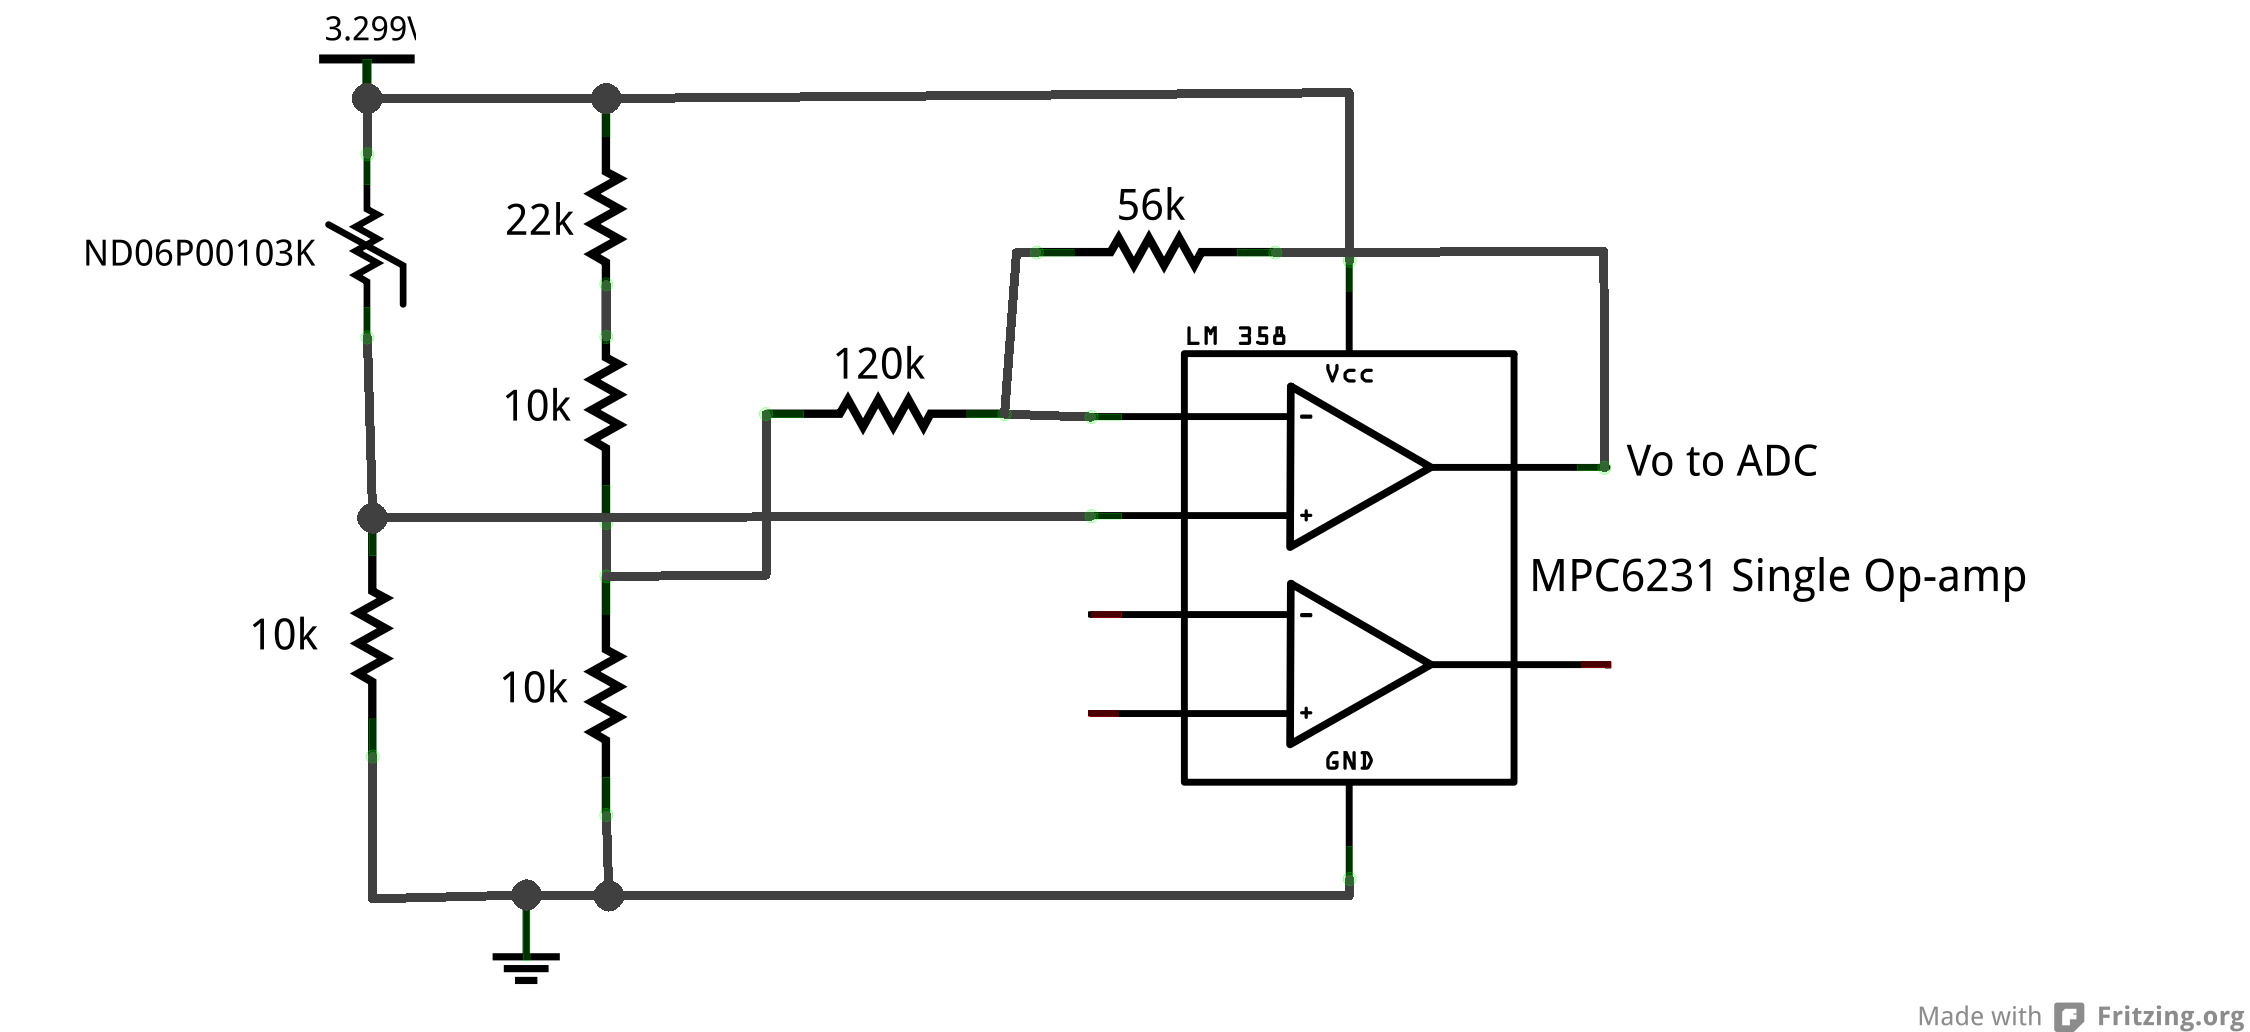
\includegraphics[width=1.0\textwidth]{Thermistor_Conditioning_nonotes_schem.png}
  \end{center}
  \caption{Temperature monitoring circuit.}
  \label{fig:tempcct}
\end{figure}

\subsection{datalogger.h}

\lstinputlisting{datalogger.h}

\subsection{datalogger.cpp}

\lstinputlisting{datalogger.cpp}

\subsection{comms.h}

\lstinputlisting{comms.h}

\subsection{comms.cpp}

\lstinputlisting{comms.cpp}

\subsection[rs232.h]{rs232.h (not written by me!)}

\lstinputlisting{rs232.h}

\subsection[rs232.cpp]{rs232.cpp (not written by me!)}

\lstinputlisting{rs232.cpp}

\FloatBarrier

\section{First Interim Report}
\label{sec:first-interim-report}

\section{Marketing Datasheet}
\label{sec:marketing-datasheet}

\bibliographystyle{plain}
\bibliography{Final_Report_Andy}

\end{document}
